\begin{figure}[H]
  \centerline{
    \begin{subfigure}{0.55\textwidth}
      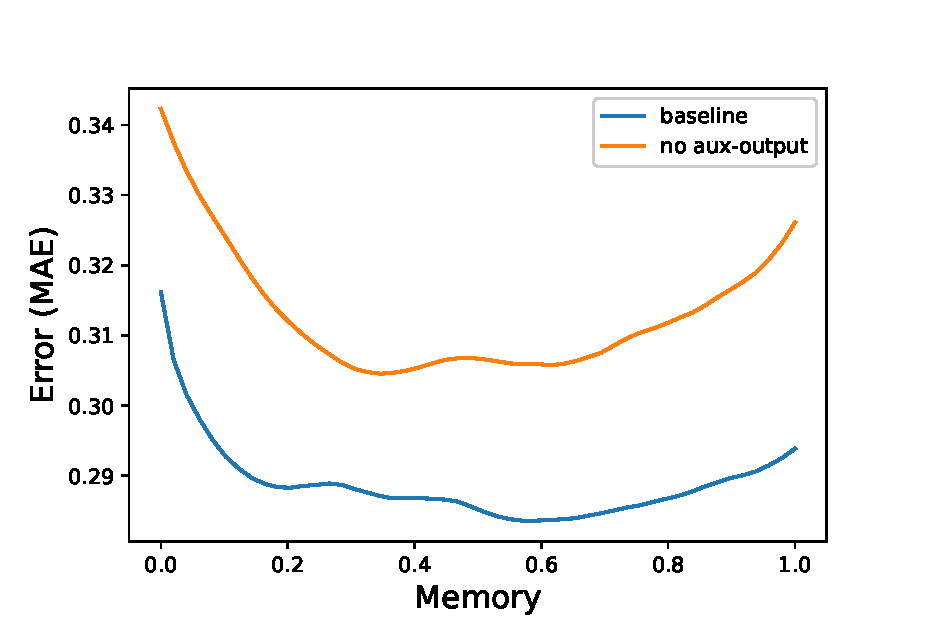
\includegraphics[width=\textwidth]{./img/comparison-sigma1.eps}%
      \caption{Deviazione standard \(\sigma=1\)}
      \label{fig:sigma1}
    \end{subfigure}
    ~
    \begin{subfigure}{0.55\textwidth}
      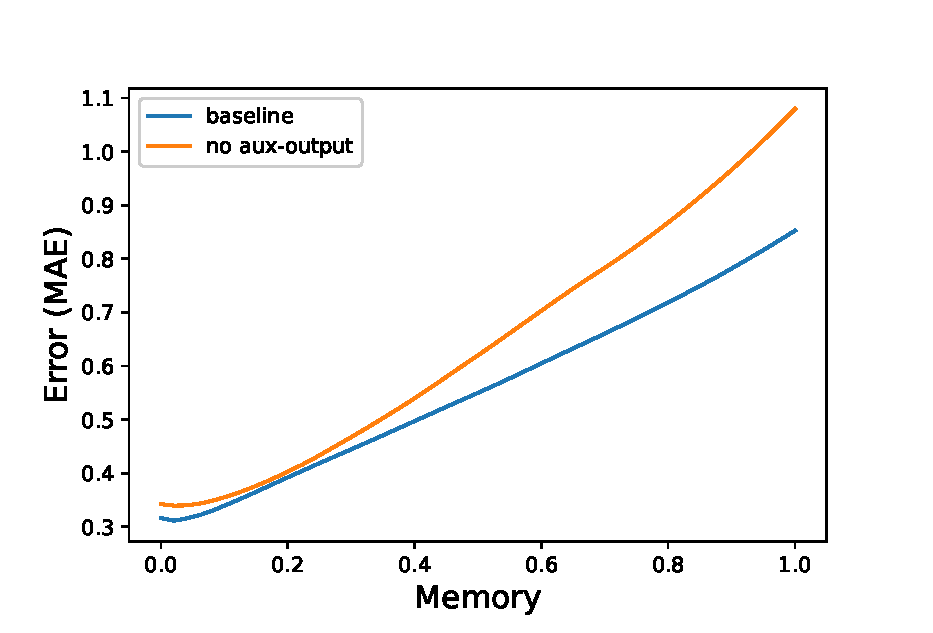
\includegraphics[width=\textwidth]{./img/comparison-sigma5.eps}%
      \caption{Deviazione standard \(\sigma=5\)}
      \label{fig:sigma5}
    \end{subfigure}
  }%
  \caption{Analisi dell'utilizzo dell'output ausiliario: i grafici mostrano
  l'andamento dell'errore (MAE) commesso dai due modelli sul dataset di test al
  variare del coefficiente di memoria residua. La curva blu rappresenta il
  modello finale, mentre la curva arancione indica il modello senza output
  ausiliario (cioè in cui \(c_1 = 0\)). Nel grafico a  sinistra, l'input
  della posizione precedente (\(\yold\)) è perturbato con del rumore
  gaussiano la cui deviazione standard è pari a \(\sigma=1\). A destra invece
  \(\sigma=5\). L'input perturbato determina una stima meno precisa dell'ultima
  posizione nota dell'utente e, con il crescere del coefficiente di memoria
  residua, entrambi i modelli tendono a sovrastimare l'importanza di tale
  input. Tuttavia, come si evince dai grafici, l'errore commesso dal modello
  \emph{baseline} cresce più lentamente ed è sempre minore di quello commesso
  dal modello senza output ausiliario.}%
  \label{fig:noauxcompare}%
\end{figure}
